\chapter{Requirement Specification}
\subsection{Introduction}
This chapter will describe the requirements needed for the multichannel audio/video playback system called Showman. This chapter contains an introductory overview of Showman in general that covers a System Description, System Overview and Usage Situation followed by Functional and Non-Functional Requirements. The chapter ends with a MoSCoW- and FURPS-analysis to organize a list of priorities needed to develop a functional prototype. \newline

\subsection{System Description}

The purpose of Showman is to play back prerecorded audio- and video-material during a concert performance. Prerecorded audio- and video-playback material  is colloquially called 'backing tracks'. The primary reason of backing track usage is to enhance a concert performance by play back additional material that artists on stage do not have the option or time to play themselves. \newline

User (or artist) uploads synchronized audio files in 44.1 kHz 16-bit .WAV-format and video files in MPEG-4 format to Showman before using Showman during showtime. User creates, edits and organizes playlist with a software application Graphical User Interface (GUI) on laptop (PC or Mac). The content of the playlist is the backing track material that user produced beforehand. After playlist creation, user uploads the playlist via a USB-connection to Showman's internal memory. \newline

Showman play back 8-tracks of audio along with video-content. The audio tracks can be connected directly into the XLR-inputs of a live sound mixer through Showman's XLR outputs, while the video-material can be connected to screens through Showman's HDMI-output.
User starts each song in the playlist separately by pressing the `Play'-button on Showman. The first song on the playlist begins and playback stops automatically (auto-stop) after each ending of a song. \newline

\begin{figure}[htb!]
\centering
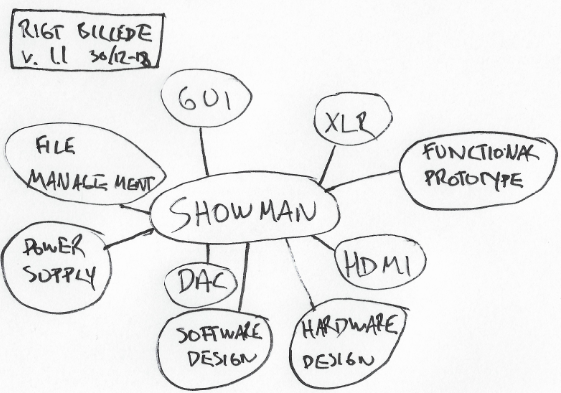
\includegraphics[scale=1]{./pictures/RigtBillede.png}
\caption{Content of Showman as a rich picture.}
\label{fig:RigtBillede.png}
\end{figure}

%\subsection{System Overview}

\subsection{Usage Situation} 

Showman's intended users are artists that utilize backing tracks at concert performances to enhance/augment their performance. Preconditions are essential to Showman, as user must have up to 4 stereo or 8 mono .WAV-files and a MPEG4-videofile available for each song that has backing tracks. The artist need to have produced the backing tracks beforehand. \newline

As Showman's intended usage conditions are tough touring conditions and periodic hard handling, Showman's user interface is a 2U 19'' rack mounted device with a LCD screen for user monitoring and panel buttons for navigation.   \newline

When the user have the necessary files available, the user assembles the playlist in the software application GUI and assigns the audio outputs. The GUI uploads the playlist project into specific folders in Showman's internal 500 GB flash memory. \newline

When user need to start playback of a song, all user need to do is press `Play' on the user panel. An auto-stop function after the end of each song in the project is embedded in Showman. \newline

\subsection{Actor-Context Diagram}

The figure below is an overview of actors that interact with Showman:

\begin{figure}[htb!]
\centering
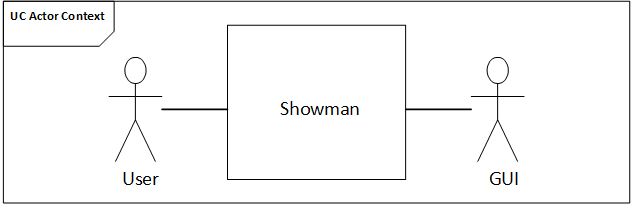
\includegraphics[scale=1]{./pictures/ActorContext.png}
\caption{Actor-Context diagram of Showman.}
\label{fig:ActorContext.png}
\end{figure}

\subsubsection{User}
User is the primary actor. User creates the playlist and uploads the playlist to Showman. User operates Showman. User's interaction with Showman is outlined in detail in the specification for the individual Use Cases. \newline

\subsubsection{GUI}
The Graphical User Interface (GUI) is the secondary actor. The GUI is the software application that handles the file management and playlist creation that is uploaded to Showman's interaction with Showman is outlined in detail in the specification for the individual Use Cases. \newline

\subsection{Functional Requirements}
This section presents the functional requirements outlined for Showman. The figure below presents a Use-Case diagram that displays the actors' relations to the Use-Cases followed by Fully Dressed Use-Cases. \newline

To keep this document brief and concise, only the first Use-Case is included. The additional Use-Cases will be explored further in the bachelor project.

%\subsubsection{Use-Case Diagram}

\subsubsection{Use-Case 1}

\begin{figure}[H]
\centering
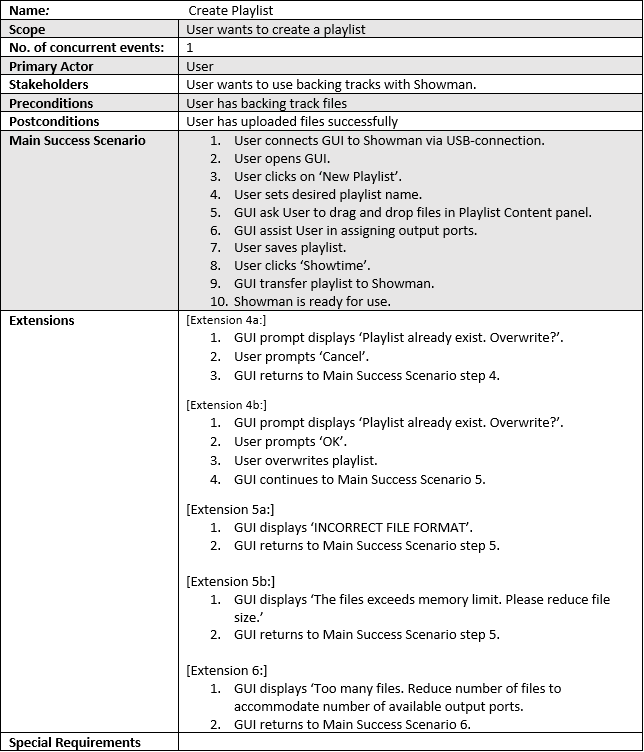
\includegraphics[scale=1]{./pictures/UC1.png}
\caption{Use-Case diagram of Use-Case 1.}
\label{fig:UC1.png}
\end{figure}

%\subsubsection{Use-Case 2}


%\subsubsection{Use-Case 3}


%\subsubsection{Use-Case 4}


%\subsubsection{Use-Case 5}


\subsection{Non-Functional Requirements}
Non-Functional Requirements (NFRs) are quality-demands, which are the qualities or constraints on the services of the functions offered by the system rather than a specific behaviour. Qualities are properties or characteristics of the system that its stakeholders care about and hence will affect their degree of satisfaction with the system. \\
Quality demands/NFRs should satisfy two attributes: \\
- Must be verifiable - e.g. measurable metrics.
- Should be objective. \newline

The NFRs are drawn up using two techniques: FURPS and MoSCoW to determine system requirements and to prioritize and rank Non-Functional Requirements. \\

\subsection{FURPS+}
FURPS+ is an acronym that represents a model classify a product's properties: \textbf{F}unctionality, \textbf{U}sability, \textbf{R}eliability, \textbf{P}erformance, \textbf{S}upportability and \textbf{+} (Design and Physical constraints, Interfaces, Legal, Test, Reuse, Economic constraints, Aesthetics, Comprehensibility, Techology tradeoff, etc.)  \\

\subsubsection{\textbf{F} - Functionality}
The functionality describes the capability (size and generality of feature set), reusability (combability, interoperability, portability) and security (safety and exploitability) of a system. \\

\subsubsection{\textbf{U} - Usability}
The usability describes the human factors, aesthetics, consistency, documentation and responsivenes of the system. \\

\subsubsection{\textbf{R} - Reliability}
The reliability describes the availability (failure frequency, robustness/durability/resilience, failure extent and time-length (recoverability/survivability), predictability (stability) and accuracy (frequency or severity of error) of the system. \\

\subsubsection{\textbf{P} - Performance}
The performance describes the speed, efficiency, resource consumption (power, RAM, cache, etc.), throughput, capacity, scalability of the system. \\

\subsubsection{\textbf{S} - Supportability
The supportability describes the serviceability, mantainability, sustainability, repair speed, testability, flexibility (modifiability, configurability, adaptabilit, extenxsibility, modularity), installability and localizability of the system. \\

\subsubsection{\textbf{?} - Design constraints}
The “+” of the FURPS+ acronym allows us to specify constraints, including design, implementation, interface, and physical constraints. \\

{\textbf{Design Constraints} – A design constraint, as the name implies, limits the design — for example, requiring a relational database stipulates the approach that we take in developing the system. \\

{\textbf{Implementation Constraints} – An implementation constraint puts limits on coding or construction – standards, platform, or implementation language. \\

{\textbf{Interface Constraints} – An interface constraint is a requirement to interact with an external item. When you develop within an enterprise, quite often you have to interact with external systems. \\

{\textbf{Physical Constraints} – Physical constraints affect the hardware used to house the system – for example, shape, size, and weight. \\

\subsection{MoSCoW}


